\documentclass[
	12pt,
	a4paper,
	bibtotoc,
	cleardoubleempty, 
	idxtotoc,
	ngerman,
	openright
	final,
	listof=nochaptergap,
	]{scrbook}

\usepackage[T1]{fontenc}
\usepackage[utf8]{inputenc}

% ##################################################
% Unterstuetzung fuer die deutsche Sprache
% ##################################################
\usepackage{ngerman}
\usepackage[ngerman]{babel}

% ##################################################
% Dokumentvariablen
% ##################################################
\newcommand{\docOrt}{Furtwangen}
\newcommand{\docTitle}{Access Point und Router mit embedded Board Banana Pi R1}
\newcommand{\docUntertitle}{}
\newcommand{\docArtDerArbeit}{Projektarbeit}
\newcommand{\docFakultaet}{Informatik}
\newcommand{\docReferent}{}
\newcommand{\docAbgabedatum}{??.??.2017}

% ##################################################
% Allgemeine Pakete
% ##################################################

% Abbildungen einbinden
\usepackage{graphicx}

% Zusaetsliche Sonderzeichen
\usepackage{dingbat}

% Farben
\usepackage{color}
\usepackage[usenames,dvipsnames,svgnames,table]{xcolor}

% Maskierung von URLs und Dateipfaden
\usepackage[hyphens]{url}

% Deutsche Anfuehrungszeichen
\usepackage[babel, german=quotes]{csquotes}

% Pakte zur Index-Erstellung (Schlagwortverzeichnis)
\usepackage{index}
\makeindex

% Ipsum Lorem
% Paket wird nur für das Beispiel gebraucht und kann gelöscht werden
\usepackage{lipsum}

% ##################################################
% Seitenformatierung
% ##################################################
\usepackage[
	portrait,
	bindingoffset=1.5cm,
	inner=2.5cm,
	outer=2.5cm,
	top=3cm,
	bottom=2cm,
	%includeheadfoot
	]{geometry}

% ##################################################
% Kopf- und Fusszeile
% ##################################################

\usepackage{fancyhdr}

\pagestyle{fancy}
\fancyhf{}
\fancyhead[EL,OR]{\sffamily\thepage}
\fancyhead[ER,OL]{\sffamily\leftmark}

\fancypagestyle{headings}{}

\fancypagestyle{plain}{}

\fancypagestyle{empty}{
  \fancyhf{}
  \renewcommand{\headrulewidth}{0pt}
}

%Kein "Kapitel # NAME" in der Kopfzeile
\renewcommand{\chaptermark}[1]{
	\markboth{#1}{}
   	\markboth{\thechapter.\ #1}{}
}

% ##################################################
% Schriften
% ##################################################

% Stdandardschrift festlegen
\renewcommand{\familydefault}{\sfdefault}

% Standard Zeilenabstand: 1,5 zeilig
\usepackage{setspace}
\onehalfspacing 

% Schriftgroessen festlegen
\addtokomafont{chapter}{\sffamily\large\bfseries} 
\addtokomafont{section}{\sffamily\normalsize\bfseries} 
\addtokomafont{subsection}{\sffamily\normalsize\mdseries} 
\addtokomafont{subsubsection}{\sffamily\normalsize\mdseries} 
\addtokomafont{caption}{\sffamily\normalsize\mdseries} 

% ##################################################
% Inhaltsverzeichnis / Allgemeine Verzeichniseinstellungen
% ##################################################

\usepackage{tocloft}

% Punkte auch bei Kapiteln
\renewcommand{\cftchapdotsep}{3}
\renewcommand{\cftdotsep}{3}

% Schriftart und -groesse im Inhaltsverzeichnis anpassen
\renewcommand{\cftchapfont}{\sffamily\normalsize}
\renewcommand{\cftsecfont}{\sffamily\normalsize}
\renewcommand{\cftsubsecfont}{\sffamily\normalsize}
\renewcommand{\cftchappagefont}{\sffamily\normalsize}
\renewcommand{\cftsecpagefont}{\sffamily\normalsize}
\renewcommand{\cftsubsecpagefont}{\sffamily\normalsize}

%Zeilenabstand in den Verzeichnissen einstellen
\setlength{\cftparskip}{.5\baselineskip}
\setlength{\cftbeforechapskip}{.1\baselineskip}

% ##################################################
% Abbildungsverzeichnis und Abbildungen
% ##################################################

\usepackage{caption}

\usepackage{wrapfig}

% Nummerierung von Abbildungen
\renewcommand{\thefigure}{\arabic{figure}}
\usepackage{chngcntr}
\counterwithout{figure}{chapter}

% Abbildungsverzeichnis anpassen
\renewcommand{\cftfigpresnum}{Abbildung }
\renewcommand{\cftfigaftersnum}{:}

% Breite des Nummerierungsbereiches [Abbildung 1:]
\newlength{\figureLength}
\settowidth{\figureLength}{\bfseries\cftfigpresnum\cftfigaftersnum}
\setlength{\cftfignumwidth}{\figureLength}
\setlength{\cftfigindent}{0cm}

% Schriftart anpassen
\renewcommand\cftfigfont{\sffamily}
\renewcommand\cftfigpagefont{\sffamily}

% ##################################################
% Tabellenverzeichnis und Tabellen
% ##################################################

% Nummerierung von Tabellen
\renewcommand{\thetable}{\arabic{table}}
\counterwithout{table}{chapter}

% Tabellenverzeichnis anpassen
\renewcommand{\cfttabpresnum}{Tabelle }
\renewcommand{\cfttabaftersnum}{:}

% Breite des Nummerierungsbereiches [Abbildung 1:]
\newlength{\tableLength}
\settowidth{\tableLength}{\bfseries\cfttabpresnum\cfttabaftersnum}
\setlength{\cfttabnumwidth}{\tableLength}
\setlength{\cfttabindent}{0cm}

%Schriftart anpassen
\renewcommand\cfttabfont{\sffamily}
\renewcommand\cfttabpagefont{\sffamily}

% Unterdrueckung von vertikalen Linien
\usepackage{booktabs}

% ##################################################
% Listings (Quellcode)
% ##################################################

\usepackage{listings}
\lstset{
	language=java,
	backgroundcolor=\color{white},
	breaklines=true,
	prebreak={\carriagereturn},
 	breakautoindent=true,
 	numbers=left,
 	numberstyle=\tiny,
 	stepnumber=2,
 	numbersep=5pt,
 	keywordstyle=\color{blue},
   	commentstyle=\color{green},   
   	stringstyle=\color{gray}
}
  	
% ##################################################
% Theoreme
% ##################################################
  	
% Umgebung fuer Beispiele
\newtheorem{beispiel}{Beispiel}

% Umgebung fuer These
\newtheorem{these}{These}

% Umgebung fuer Definitionen
\newtheorem{definition}{Definition}
  	
% ##################################################
% Literaturverzeichnis
% ##################################################

\usepackage{bibgerm}

% ##################################################
% Abkuerzungsverzeichnis
% ##################################################

\usepackage[printonlyused]{acronym}

% ##################################################
% PDF / Dokumenteninternelinks
% ##################################################

\usepackage[
   	linkcolor=black,
   	citecolor=black,
  	filecolor=black,
	urlcolor=black,
    bookmarks=true,
    bookmarksopen=true,
    bookmarksopenlevel=3,
    bookmarksnumbered,
    plainpages=false,
    pdfpagelabels=true,
    hyperfootnotes,
    pdftitle ={\docTitle}]{hyperref}


\begin{document}

\setcounter{secnumdepth}{3}

% Titelblatt
\begin{titlepage}
\pagestyle{empty}

% ##################################################
% HFU-Logo einbinden
% ##################################################
\begin{flushright}
\begin{figure}[ht]
\flushright

\includegraphics[height=3cm]{pictures/hfu.jpg}
\end{figure}
\end{flushright}

% ##################################################
% Titel
% ##################################################
\begin{center}
{\fontsize{18}{22} \selectfont \docArtDerArbeit}\\[5mm]
{\fontsize{18}{22} \selectfont in der Fakult\"at} \\[5mm]
{\fontsize{18}{22} \selectfont \docFakultaet}\\
\vspace{1cm}
\begin{onehalfspace}
{\fontsize{22}{26} \selectfont \textbf{\docTitle}}\\[5mm]
{\fontsize{18}{22} \selectfont \docUntertitle}


\end{onehalfspace}
\end{center}

% ##################################################
% Zusatzinformationen
% ##################################################
\vfill
\begin{center}
\begin{tabular}{lcl}
Referent	&:& Dr. Jiri Spale	\\ \\
Vorgelegt am 	&:& \docAbgabedatum 	\\ \\
Vorgelegt von 	&:& Bastian	\\
		& & Elias	\\
		& & Jakob	\\
		& & Jonas	\\
		& & Tom
\end{tabular}
\end{center}
\end{titlepage}

\cleardoubleemptypage

\frontmatter


% Abstract
\chapter*{Abstract\markboth{Abstract}{}}
\addcontentsline{toc}{chapter}{Abstract}

The project „Access Point und Router mit embedded Board Banana Pi R1“ is a continuation of a previous project done at the university in Furtwangen of the same name from the winter semester 2016/2017. Its main goals were to find a suitable operating system for the BananaPi and recording the network traffic. There were future objectives listed at the end of the documentation which have been worked upon in this semester. The main goals for this project are to further analyse and test applicable operating systems as well as implementing different functions such as Radius, Samba, Mailserver, display status readout and a backup solution.
\\\\\\
Bei dem Projekt „Access Point und Router mit embedded Board Banana Pi R1“, handelt es sich um die Weiterführung des bereits im Wintersemester 2016/2017 an der Hochschule Furtwangen abgehaltenen Projekts mit demselben Name. Das damalige Vorhaben bestand daraus, ein passendes Betriebssystem für den BananaPi zu ermitteln und den Netzwerkverkehr aufzuzeichnen. Am Ende wurden zukünftige Ziele aufgelistet welche in diesem Semester erarbeiten wurden. Projektziele sind, das Analysieren und Testen passender Betriebssysteme, sowie die Implementierung verschiedener Funktionen wie Radius, Samba, einem Mailserver, einer Displaystatusanzeige und einer Backup Lösung.

\cleardoubleemptypage

% Inhaltsverzeichnis
\tableofcontents
\addcontentsline{toc}{chapter}{Inhaltsverzeichnis}
\cleardoubleemptypage

% Abbildungsverzeichnis einbinden und ins Inhaltsverzeichnis
% WORKAROUND: tocloft und KOMA funktionieren zusammen nicht
% korrekt\phantomsection
\addcontentsline{toc}{chapter}{\listfigurename} 
\listoffigures
\cleardoubleemptypage

% Tabellenverzeichnis einbinden und ins Inhaltsverzeichnis
% WORKAROUND: tocloft und KOMA funktionieren zusammen nicht
% korrekt\phantomsection
%\phantomsection
%\addcontentsline{toc}{chapter}{\listtablename}
%\listoftables
%\cleardoubleemptypage

% Abkürzungsverzeichnis
\chapter*{Abkürzungsverzeichnis\markboth{Abkürzungsverzeichnis}{}}
\addcontentsline{toc}{chapter}{Abkürzungsverzeichnis}

\begin{acronym}
\acro{HFU}{Hochschule Furtwangen University}
\acro{PSW}{Pumpspeicherwerk}
\end{acronym}

\mainmatter

\chapter{Projektübersicht}

\section{Kontext}
Das Projekt mit dem Titel Router mit embedded Board Banana Pi R1 wird als Se-
mesterprojekt im Sommersemester 2017 an der Hochschule Furtwangen durch-
geführt. Das Projekt wurde von Dr. Jiri Spale ins Leben gerufen und wird
intern, ohne die Kooperation mit einem Unternehmen durchgeführt. Die Anzahl der studentischen Projektteilnehmer beträgt fünf.

\section{Ziel}
Das primäre Ziel des Projektes ist es, das bestehende Router-Projekt weiterzuentwickeln. Folgende Funktionalitäten sollen implementiert werden:\\
~\\
\begin{itemize}
\item Implementierung eines RADIUS-Servers zur zentralen Authentifizierung von Anwendern
\item Implementierung einse Voucher-Systems
\item Installation des Betriebssystems IP Fire
\item Mehrere WLAN Access Points auf einem WLAN-Chip
\item Mail-Server zum Statusbericht der Backups
\item SAMBA/NFS Server
\item Automatische Aktuatisierung von Programmpaketen des Systems
\item Implementierung einer Display-Statusanzeige
\end{itemize}
~\\
Die Funktionen sollen auf dem Betriebssystem “Bananian”, ein auf das Banana Pi zugeschnittenes Debian, implementiert werden.

\chapter{Betriebssystemübersicht}

Zu Begin des Projektes standen die beiden Betriebssysteme OpenWRT und Bananian zur Verfügung.
Außerdem gab es den Vorschlag des VorgängerProjekts, zusätzlich das Projekt auch mit dem Betribssystem IPFire durchzuführen.
Die Nutzung der einzelnen Betriebssysteme fiel sehr unterschiedlich aus, da die implementierten Funkionen und der Stand der Entwicklung sich stark von System zu System unterschied.

\section{OpenWRT}
OpenWRT ist ein Betriebssystem, das für eingebettete Geräte wie Wlan Router enwickelt wurde.
Das System wird übe ein Webinterface angepasst und unterscheidet sich stark zu den anderen im Projekt verwendeten Betriebssystemen.
Durch diese Unterschiede wurden nur enzelne Teile des Projektes auf OpenWRT umgesetzt.

\section{IPFire}
\begin{wrapfigure}{r}{5cm}
\centering

\includegraphics[width=3.5cm]{pictures/Jakob/IPFire}
\caption{IPFire Logo}
Quelle: \cite{fire1}
\end{wrapfigure}
Das Betriebssystem IPFire ist darauf ausgelegt, als Router genutzt zu werden, wobei das Augenmerk auf der implementierung einer Firewall oder eines VPN Gateways liegt.
Das vorgehende Projekt hatte dieses Betriebssystem als Alternative vorgeschlagen, weshalb wir dieses System als Aternative untersucht haben. Zwei Abbilder für den Betrieb auf Arm Prozessoren stehen auf der Webseite des Betriebssystems bereit. \cite{fire} \\
Bei beide Abbildern stellte sich allerdings herraus, dass die HDMI Schnittstelle nicht unterschtützt wird.
Auch eine Verbindung SSH nicht möglich ist, da IPFire auf eine Konfiguration über das Webinterface ausgelegt ist.
Eines der beiden Abbilder ist auf die Konfiguration über eine Serielle Schnittstelle Ausgelegt. Da uns aber für diese Schnittstelle keine Wekzeuge und Adapter bereitstehen, haben wir auch von dieser Option abgelassen.\\

\newpage
\section{Bananian}
\begin{wrapfigure}{r}{5cm}
\centering

\includegraphics[width=3cm]{pictures/Jakob/Bananian}
\caption{Bananian Logo}
Quelle: \cite{bananian1}
\end{wrapfigure}
Der Banana Pi R1 wird von dem Betribssystem Bananian vollständig unterstützt. Dieses Betriebssystem basiert auf Debian 8 und nutzt das Debian Jessie armhf repositorie. \cite{bananian}\\
Neben OpenWRT wurde das Projekt mit Bananian gestartet. Da die Weiterentwicklung von Bananian am 2.4.2017 eingestellt wurde haben wir uns einschieden auf das Betriebssystem Armbian zu wechseln. \cite{bananian2}

\section{Armbian}
\begin{wrapfigure}{r}{5cm}
\centering

\includegraphics[width=3.5cm]{pictures/Jakob/Armbian}
\caption{Armbian Logo}
Quelle: \cite{armbian}
\end{wrapfigure}
Wie auch Bananian basiert Armbian auf Debian Jessie, das speziell für ARM Prozessoren entwickelt wurde. Dieses Betriebssystem haben wir gewählt, da es Bananien stark ähnelt, im Gegensatz zu Bananian aber weiterentwickelt wird und damit auch in gewissem Maße für die Zukunft gewappnet ist. Außerdem unterstützt es alle Funktionen die für das Projekt benötigt werden. \cite{armbian1}








\chapter{Implementierung}
\section{Backup und Wiederherstellung des Betriebssystems}

Um die Implementationen und Konfigurationen des Pi's abzusichern, wird eine Backup Lösung eingesetzt. Die Sicherung relevanter Daten soll hierbei einem möglichen Defekt oder Inkompatibilität durch Updates o.ä. entgegenwirken.\\
\\
'FauBackup' und 'gitbac' bieten hierbei eine Lösung mittels externer Programme an. Debian bietet jedoch bereits standardmäßig einige Aufrufe welche zur Anlegung von Backups verwendet werden können. Diese wurden im Folgenden in Ubuntu anhand eines Bash Skripts zur Automatisierung getestet und implementiert.\\

\subsection{dd}
Als erste Ausführung wurde der Aufruf 'dd' verwendet. Hierbei wird der Inhalt der gesamten SD Karte als Image Datei abgespeichert.

\subsubsection*{Schritt 1:}
Übersicht der vorhandenen Dateisysteme mittels des Terminalaufrufs 'df'\\
\begin{figure}[ht]
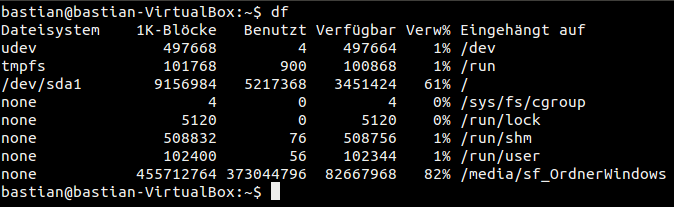
\includegraphics[width=.8\textwidth]{pictures/Bastian/BILD1_df}
\caption{Vorhandene Dateisysteme}
\end{figure}

\subsubsection*{Schritt 2:}
Terminalaufruf für den Backupprozess
\lstset{language=bash,numbers=none,frame=single}
\begin{lstlisting}
sudo dd if=INPUTPARTITION of=OUTPUTFILE
\end{lstlisting}
\begin{tabular}{l c l}
sudo	& -> & Backupprozess benötigt root-Rechte\\
dd	& -> & bit-genaues Kopieren der Dateien\\
if=FILE	& -> & Die Datei oder Partition welche integriert wird\\
of=FILE & -> & Die Output Datei welche angelegt wird\\
\end{tabular}
\newpage %==============================================

\subsubsection*{Schritt 3:}
Optionale Nutzung von Terminalaufruf 'pv' um den Fortschritt des Backup Prozesses zu sehen Die mögliche Restzeit lässt sich nur durch das Hinterlegen der Größe der Partition anzeigen.
\begin{lstlisting}
sudo dd if=INPUTPARTITION |pv| sudo dd of=OUTPUTFILE
\end{lstlisting}
\begin{figure}[ht]
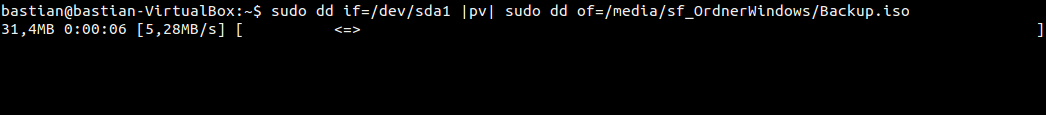
\includegraphics[width=\textwidth]{pictures/Bastian/BILD2_pv}
\caption{Laufender Backupprozess mit Statusanzeige}
\end{figure}
\subsubsection*{Schritt 4:}
Wiederherstellen eines hinterlegten Backups läuft ähnlich wie der ursprüngliche Prozess ab.
\begin{lstlisting}
sudo dd if=OUTPUTFILE |pv| of=INPUTPARTITION
\end{lstlisting}
\begin{figure}[ht]
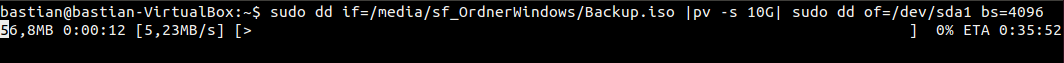
\includegraphics[width=\textwidth]{pictures/Bastian/BILD3_pv}
\caption{Laufender Wiederherstellungsprozess mit Statusanzeige}
\end{figure}
Quelle: https://wiki.ubuntuusers.de/dd/ \cite{dd}
\newpage %==============================================

\subsection{rsync}
Da der Vorgang mittels 'dd' als suboptimal angesehen wird, wurde alternativ der Aufruf 'rsync' verwendet. Dieser bietet die Möglichkeit eines inkrementellen Backups wodurch die Dauer des Prozesses erheblich reduziert werden kann. Hierbei werden die Größe und die Änderungszeit der Dateien in Quelle und Ziel miteinander verglichen. Eine Aktualisierung findet demnach nur statt, wenn Unterschiede vorzufinden sind.
\begin{lstlisting}
rsync -aAXv --delete --exclude={"/dev/*","/proc/*","/sys/*","/tmp/*","/run/*","/mnt/*","/media/*","/lost+found"} / /path/to/backup/folder
\end{lstlisting}
\begin{tabular}{l c l}
rsync	&->& Kopieren der Dateien\\
-aAX	&->& Übertragung im Archiv Modus wodurch alle symbolischen Verweise\\
	&  & beibehalten werden\\
--delete&->& Dateien die im Ursprungsverzeichnis nicht mehr existieren werden\\
	&  & im Zielverzeichnis ebenfalls gelöscht\\
--exclude&->& Dateien werden ausgelassen\\
\end{tabular}\\\\
Wiederherstellen des Rsync Backups durch folgenden Befehl:
\begin{lstlisting}
rsync -aAXv /path/to/backup/location/* /mount/point/of/new/install/ --exclude={/dev/*,/proc/*,/sys/*,/tmp/*,/run/*,/mnt/*,/media/*,/lost+found,/home/*}
\end{lstlisting}
Quelle: https://wiki.ubuntuusers.de/rsync/ \cite{rsync}
\subsection{tar} %===============================================================================
Eine weitere Anwendungsmöglichkeit bietet die 'tar' Archivierung. Vorteil dieses Aufrufs ist, dass durch Angabe von Parametern die Berechtigungen aller zu sichernden Daten ebenfalls beibehalten werden und die Archivierung Speicherplatz spart.\\
Wechsel in das Backupverzeichnis dann:
\begin{lstlisting}
tar -cpzf Backup.tar ORDNER
\end{lstlisting}
\begin{tabular}{l l}
tar	&-> Archivieren von Daten\\
-c	&-> Archiv wird erzeugt (create)\\
-p	&-> Berechtigungen beibehalten (privilige)\\
-z	&-> Zusätzliche Komprimierung mit gzip\\
-f	&-> Archiv in Datei schreiben (finish)\\
\end{tabular}
 ~\\Quelle: https://wiki.ubuntuusers.de/tar/ \cite{tar}

\newpage %==============================================

\subsection{Automatisierung mittels Bash-Skript} %===============================================
Damit der Nutzer die Aufrufe nicht händisch zu bestimmten Zeiten ausführen muss, wurden zwei Bash-Skripte zur Automatisierung geschrieben. Es gibt ein monatliches Backup mittels (tar) und wöchentliche inkrementelle Backups (rsync) auf die zurückgegangen werden kann.\\
\\
Um das Zeitintervall der Backups einzustellen wird der 'Cron' Dienst verwendet.
Hiermit können Skripte und Programme zu festgelegten Zeiten gestartet werden.
Wenn ein hinterlegter Job täglich zu einer bestimmten Uhrzeit ausgeführt wird muss allerdings auch der Rechner zu dem Zeitpunkt aktiv sein. Ist dies nicht der Fall, startet der Prozess nicht. Um dies zu umgehen wird 'Anacron' verwendet.
Durch ablegen des Skripts in eines der entsprechenden Verzeichnisse wird der Prozess entsprechend ausgeführt.\\
Quelle: https://wiki.ubuntuusers.de/Cron/ \cite{cron} \\
\begin{tabular}{l l}
/etc/cron.hourly/	&- Stündlich ausführen\\
/etc/cron.daily/	&- Täglich ausführen\\
/etc/cron.weekly/	&- Wöchentlich ausführen\\
/etc/cron.monthly/	&- Monatlich ausführen\\
\end{tabular}
\begin{figure}[ht]
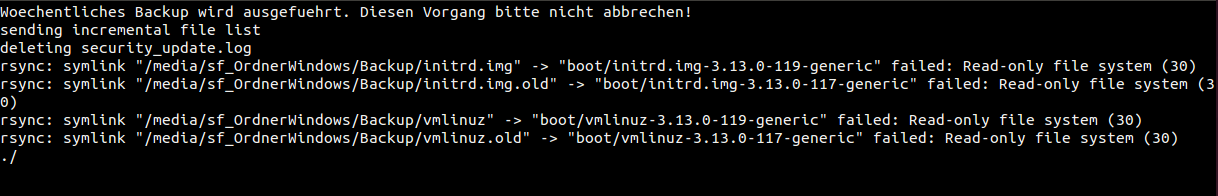
\includegraphics[width=\textwidth]{pictures/Bastian/Woechentliches_Backup}
\caption{Ausführung wöchentliches Backup}
\end{figure}

\section{Update des Banana Pi}
Ziel war es das Betriebssystem und alle Programme immer auf dem aktuellsten Stand zu halten. Hierbei kann es jedoch zu Inkompatibilität bestimmter Funktionen  oder Konfigurationen kommen. Daher wurde die Umsetzung auf die relevantesten Updates (Sicherheitsupdates) reduziert. Im Normalfall können mittels des Konsolenaufrufs  'apt-get update' die Updateliste und mit 'apt-get upgrade' die Programm Pakete selbst aktualisiert werden. Durch Nutzung des Aufrufs 'unattended-upgrade' wird auf Sicherheitsupdates des Systems überprüft und diese anschließend installiert.\\
\\
Durch 'unattended-upgrade --dry-run -d' wird auf Verfügbarkeit von Updates geprüft ohne anschließende Installation. Nach jedem Durchgang wird eine Logdatei in /var/log/unattended-upgrades/ angelegt welche genauere Informationen zu den aktualisierten Dateien liefert.

\section{Implementierung einer Displaystatusanzeige}
Zur besseren Übersicht des Netzwerktraffics als auch der Ressourcen des Banana Pi sollte eine Displaystatusanzeige implementiert werden. Der Aufruf 'htop' bietet eine Übersicht aller laufenden Prozesse und deren Ressourcennutzung. 'iftop' zeigt die Netzwerkinterfaces und die eingehende und ausgehende Kommunikationen. Da das Terminal jedoch nur einen der Befehle zu einem Zeitpunkt ausüben kann wird ein Terminal-Multiplexer verwendet. Zur Auswahl stehen hierbei 'Terminator', 'screen', und 'Tmux'. Aufgrund der geringen Einarbeitungszeit und einfachen Anwendbarkeit wurde letzteres zur Implementation ausgewählt. Alle Multiplexer bieten die Möglichkeit Sitzungen zu erstellen. Leider kann dies nicht zur Implementierung der Displaystatusanzeige verwendet werden, da die Sitzung beim Herunterfahren des Betriebssystems gelöscht wird. Daher wird zum Systemstart ein Bash-Skript eingesetzt, welches automatisch die benötigten Fenster zur Überwachung anlegt.
\begin{figure}[ht]
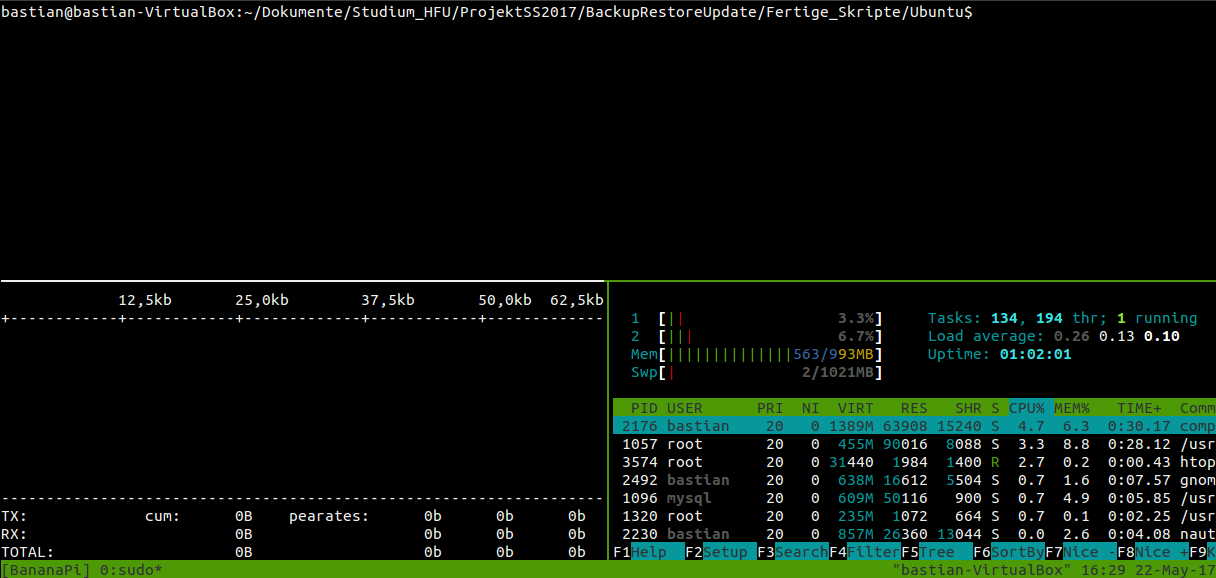
\includegraphics[width=\textwidth]{pictures/Bastian/Tmux}
\caption{Verwendung von Tmux mit 'htop' und 'iftop'}
\end{figure}


\section{Mail-Server}
Um Statusbenachrichtigungen zu erhalten, wurde ein Mail-Server auf dem Pi eingerichtet, welcher als Relay über Google Mail fungiert. Dazu wurde ein Google Mail Konto eingerichtet, auf welches Post Fix zugreift und Mails verschickt.\\
Alle System Mails werden Über das Google-Konto weitergeleitet, dazu gehören auch Statusmeldungen des Backup-Skripts.\\
Dieser Weg wurde wegen des geringen Aufwands gewählt. Ohne Relay würde man eine eigene Domain und sehr viel mehr Konfiguration benötigen. Da ein Google Mail Konto nie verfällt, war dies die beste und pflegeleichteste Möglichkeit.\\
Weiterhin können die Mails auch an jede beliebige Adresse verschickt werden, dies ist im Mail-Server frei konfigurierbar. Die Mails gehen momentan an die Google Mail Adresse.

\subsection{Einrichtung}
Voraussetzungen:\\
- Internetzugriff\\
- Google Mail-Konto\\
- Texteditor (Nano)\\
- SSH/Physikalischen Zugriff\\
~\\
1. Post Fix installieren:
\begin{lstlisting}
apt-get update
apt-get install postfix libsasl2-modules bsd-mailx
\end{lstlisting}
~\\
2. Das Konfigurationsfenster öffnet sich.\\
~\\
3. TLS/SSL aktivieren:
\begin{lstlisting}
nano /etc/postfix/main.cf
\end{lstlisting}
~\\
3.1 Folgendes Einfügen:
\begin{lstlisting}
mtp_sasl_auth_enable = yes
smtp_sasl_security_options = noanonymous
smtp_sasl_password_maps = hash:/etc/postfix/sasl_password
# verschluesselung einschalten
smtp_tls_security_level = may
\end{lstlisting}
~\\
4. Nutzerdaten des Google Mail-Kontos hinterlegen:
\begin{lstlisting}
nano /etc/postfix/sasl_password
smtp.gmail.com Bananapihfu:<Password>
\end{lstlisting}
~\\
5. Datei nur für root lesbar machen, da Klartext:
\begin{lstlisting}
chmod 600 /etc/postfix/sasl_password 
\end{lstlisting}
~\\
6. Postfix lookup Tabelle erstellen:
\begin{lstlisting}
postmap hash:/etc/postfix/sasl_password
\end{lstlisting}
~\\
7. Postfix neustarten:
\begin{lstlisting}
/etc/init.d/postfix restart
\end{lstlisting}
~\\
8. Für Weiterleitung der Systemnachrichten aliases bearbeiten:
\begin{lstlisting}
nano /etc/aliases 
root: bananapihfu@gmail.com
\end{lstlisting}
Oder Wunschemail an welche Systemnachrichten gesendet werden\\
~\\
9. Änderungen an Aliases wirksam machen:
\begin{lstlisting}
Newaliases
\end{lstlisting}





\section{Samba}
Um den Dateizugriff zu erleichtern, wurde ein Samba-Server auf dem Pi implementiert.\\
Samba ermöglicht es von nahezu jedem Gerät auf ein Freigegebenes Verzeichnis auf dem Server zuzugreifen. Voraussetzung ist, dass das Client Betriebssystem das SMB-Protokoll unterstützt.\\
Die meisten modernen Betriebssysteme, wie Windows, MacOS und andere Unixoide besitzen Samba Funktionalität.\\
~\\
Einrichtung\\
Voraussetzungen:\\
- Internetzugriff\\
- Texteditor (Nano)\\
- SSH/Physikalischen Zugriff\\
\\
1. Samba installieren:
\begin{lstlisting}
sudo apt-get update
sudo apt-get install samba
\end{lstlisting}
~\\
2. Benutzer für Samba erstellen (Hat keinen Shell-Zugriff):
\begin{lstlisting}
useradd sambausr --shell /bin/false
\end{lstlisting}
~\\
3. Passwort für den Benutzer in Samba setzen:
\begin{lstlisting}
smbpasswd -a <user_name>
\end{lstlisting}
~\\
4. Verzeichnis im Homer erstellen:
\begin{lstlisting}
mkdir /home/sambausr
mkdir /home/sambausr/samba
\end{lstlisting}
~\\
5. Berechtigungen setzen:
\begin{lstlisting}
chown sambausr:sambausr /home/sambausr/
chown sambausr:sambausr /home/sambausr/samba/
\end{lstlisting}
~\\
6. Backup der Samba Konfiguration im Homeverzeichnis machen:
\begin{lstlisting}
cp /etc/samba/smb.conf ~
\end{lstlisting}
~\\
7. Config bearbeiten:
\begin{lstlisting}
nano /etc/samba/smb.conf
\end{lstlisting}
~\\
7.1 folgendes am Ende der Konfiguration Einfügen:
\begin{lstlisting}
[samba]
path = /home/sambausr/samba
valid users = sambausr
read only = no
\end{lstlisting}
~\\
8. Service neustarten:
\begin{lstlisting}
service smbd restart
\end{lstlisting}
~\\
9. Config testen:
\begin{lstlisting}
testparm
\end{lstlisting}
~\\Quelle: https://help.ubuntu.com/community/How to Create a Network Share... \cite{samba}

\section{DDNS}
Um immer die aktuelle IP-Adresse des Pi zur Hand zu haben, wurde ein DynDNS-Client von no-ip implementiert, bei jedem Systemstart wird die bei der DNS hinterlegte IP-Adresse aktualisiert.\\
Nachteil hierbei ist jedoch, dass man alle 30 Tage diese Domain aktivieren muss, da diese sonst verfällt.\\
Um dies zu umgehen wurde die Kostenfreie Domain bananapihfu.tk gebucht. Von Vorteil ist hier, dass diese Domain eine Laufzeit von einem Jahr hat und nach Ablauf auch ohne Mehrkosten verlängert werden kann.\\
Diese Domain wird bei Cloudflare verwaltet, da hier auch eine API angeboten wird, mit welcher man Theoretisch komplett auf eine Dynamische DNS bei No-IP verzichten kann.

\subsection{Einrichtung No-IP}
Voraussetzungen:\\
- Internetzugriff\\
- SSH/Physikalischen Zugriff\\
- NoIP.com Account\\
\\
1. NoIP Hostnamen anlegen:\\
Man muss in No-IP den gewünschten Hostnamen einrichten, welcher später auf die aktuelle IP-Adresse verweist.\\
\begin{figure}[ht]
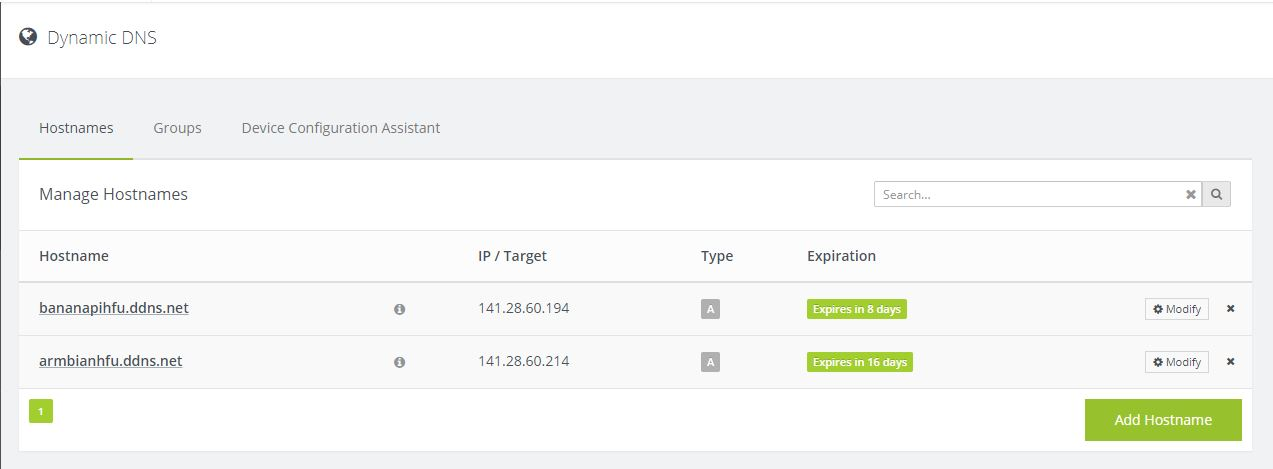
\includegraphics[width=\textwidth]{pictures/Jonas/noip_Domain}
\caption{noip Domain}
\end{figure}
~\\
2. Verzeichnis für DDNS im Homeverzeichnis erstellen und wechseln:
\begin{lstlisting}
mkdir DDNS
cd DDNS
\end{lstlisting}
~\\
3. NoIP-Client von NoIP.com beziehen:
\begin{lstlisting}
wget https://www.noip.com/client/linux/noip-duc-linux.tar.gz
\end{lstlisting}
~\\
4. Das Archiv entpacken:
\begin{lstlisting}
tar xvf noip-duc-linux.tar.gz
\end{lstlisting}
~\\
5. In den Entpackten Ordner wechseln:\\
cd noip eingeben und mit TAB vervollständigen
\begin{lstlisting}
cd noip-x.x.x-x 
\end{lstlisting}
~\\
6. Client bauen und installieren:
\begin{lstlisting}
make && make install
\end{lstlisting}
~\\
7. Konfiguration wird gestartet:
\begin{lstlisting}
Auto configuration for Linux client of no-ip.com.

Multiple network devices have been detected.

Please select the Internet interface from this list.

By typing the number associated with it.
0       eth0.101
1       eth0.201
2       eth0.202
\end{lstlisting}

0
\begin{lstlisting}

Please enter the login/email string for no-ip.com  bananapihfu
Please enter the password for user 'bananapihfu'  ***********

Only one host [armbianhfu.ddns.net] is registered to this account.
It will be used.
Please enter an update interval:[30]  30
Do you wish to run something at successful update?[N] (y/N)  N

New configuration file '/usr/local/etc/no-ip2.conf' created.
\end{lstlisting}
~\\
Um den Daemon automatisch bei Systemstart zu starten muss noch folgende Konfiguration vorgenommen werden:\\
1. Startscript unter /etc/init.d/noip2 ablegen:
\begin{lstlisting}
vim /etc/init.d/noip2
\end{lstlisting}
~\\
2. Script "noip2" kopieren und einfügen:\\
Verweis auf Anhang\\
~\\
3. Script ausführbar machen:
\begin{lstlisting}
chmod a+rx /etc/init.d/noip2
\end{lstlisting}
\newpage
\subsection{Einrichtung Custom-Domain}
Voraussetzungen:\\
- Account bei Cloudflare\\
~\\
1. Domain bei Freenom.com aussuchen:\\
Hier gibt es jede Menge kostenfreie Domains\\
~\\
2. Wunsch-Domain registrieren\\
\begin{figure}[ht]
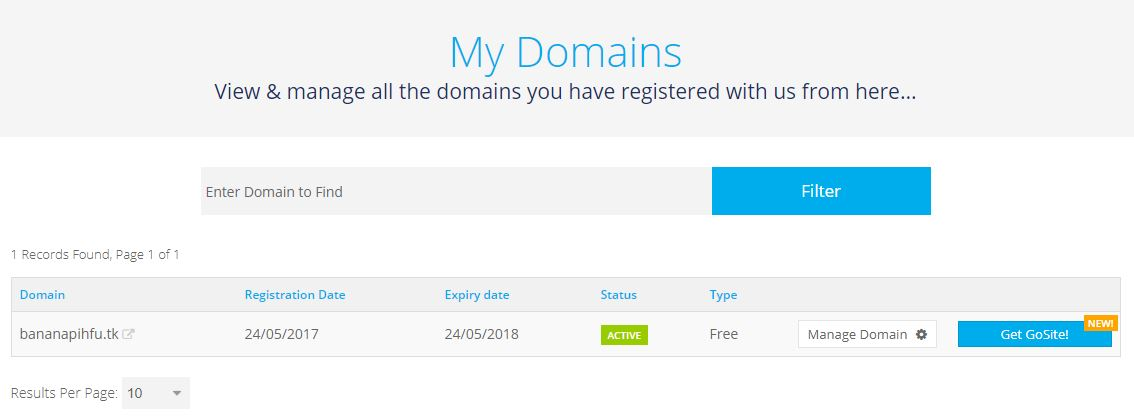
\includegraphics[width=\textwidth]{pictures/Jonas/freenom_Domain}
\caption{freenom Domain}
\end{figure}

3. Nameserver bei Freenom ändern:\\
Um die Domain bei Cloudflare zu verwalten, müssen die Nameserver angepasst werden.
Diese erhält man, wenn man sich bei Cloudflare anmeldet.\\
\begin{figure}[ht]
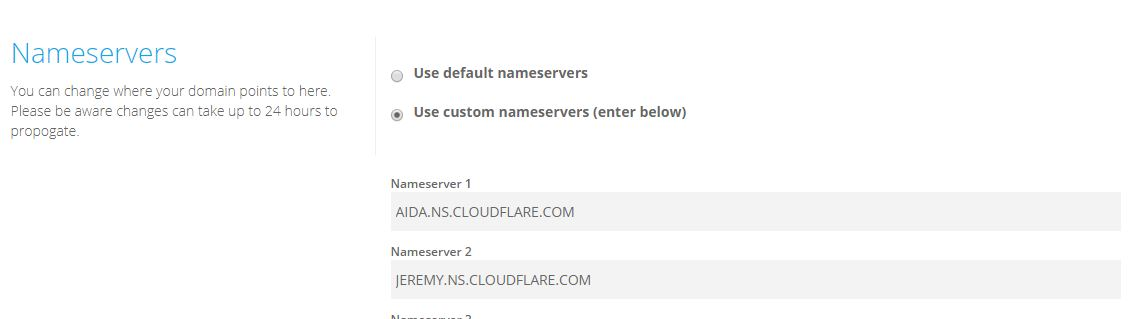
\includegraphics[width=\textwidth]{pictures/Jonas/freenom_Nameserver}
\caption{freenom Nameserver}
\end{figure}
\newpage
3. CNAME Weiterleitung auf No-Ip einrichten\\
\begin{figure}[ht]
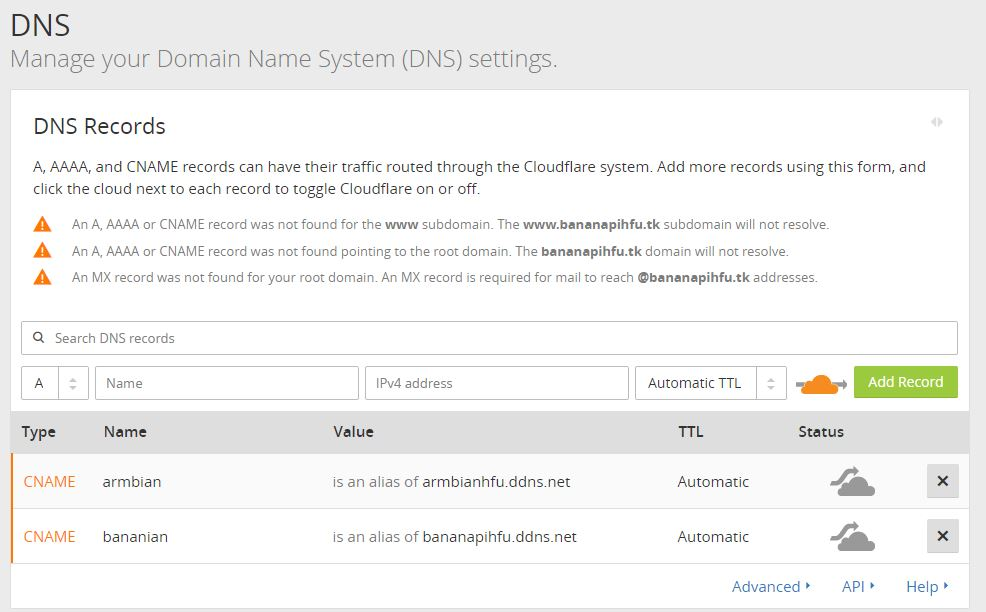
\includegraphics[width=\textwidth]{pictures/Jonas/Cloudflare_DNS}
\caption{Cloudflare DNS}
\end{figure}



\section{Radius}
\subsection{Allgemein}
Der Remote Authentication Dial-In User Service (RADIUS, deutsch Authentifizierungsdienst für sich
einwählende Benutzer) ist ein Protokoll zwischen Benutzer und Server, das für die 3 A‘s (dem
sogenannten Tripple-A-System), also der Authentifizierung, Autorisierung und das Accounting
zuständig ist.
Laut Internetquellen ist es der „De-facto Standard bei der zentralen Authentifizierung von
Einwahlverbindungen über Modem, ISDN, VPN, WLAN (IEEE 802.1X) und DSL“. \cite{rad1}

\subsection{Funktionsweise}
\begin{figure}[ht]                    
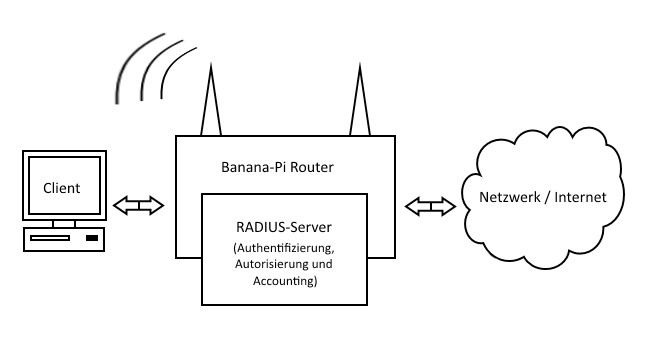
\includegraphics[width=\textwidth]{pictures/Tom/Radius}
\caption{Radius Funktionsweise}
\end{figure}
Anhand der obenstehenden Abbildung lässt sich gut erkennen wie der Aufbau ist. Der Client
(Smartphone, PC, etc.) kann sich wahlweise per WLAN oder LAN mit dem Banana-Pi Router
verbinden, dabei sendet er eine Authentifizierungsanfrage an diesen, welche der Router an den
Radius-Server, welcher auf dem Banana-Pi läuft, weiterleitet. Dieser verarbeitet nun die Anfrage
indem er, je nach Konfiguration, in unserem Fall über eine SQL-Datenbank überprüft ob der Client
berechtigt ist dem Netzwerk beizutreten. Zusätzlich kann diese Verbindung dann auch limitiert
werden (Volumen-Limit, Bandbreiten-Drosselung, beschränkter Zugriff auf Subnetze/VLANs).
\newpage

\subsection{FreeRADIUS}
FreeRADIUS ist wie der Name schon vermuten lässt eine freie und kostenlose Implementierung des
RADIUS-Protokolls und unter der GNU General Public License, version 2 lizenziert. Es ist laut
eigenen Angaben der weltweit am meisten eingesetzte RADIUS-Server und wird von den meisten
Internetdienstanbietern (Providern) sowie den 500 umsatzstärksten Unternehmen der Welt
benutzt. \cite{rad2}\\
Es findet außerdem auch in der Hochschule sowie im akademischen Forschungsnetzwerk Eduroam
Einsatz. Es unterstützt den meistverbreiteten Authentifizierungsstandard EAP, auf deutsch etwa„Erweiterbares Authentifizierungsprotokoll“ \cite{rad3}
, der ca. 40 verschiedene Verfahren anbietet, welche
heutzutage unter anderem in den Sicherheitsimplementationen WPA und WPA2 Verwendung
finden.\\
~\\
Installation:\\
FreeRADIUS ist auch in den offiziellen Paket-Quellen von Debian enthalten und kann somit ganz
einfach über den Debian-Paketmanager apt-get installiert werden. Als erstes stellen wir sicher dass
das System up-to-date ist und die aktuellen Paketquellen besitzt. \cite{rad4}
\begin{lstlisting}
sudo apt-get update
sudo apt-get upgrade
sudo apt-get freeradius freeradius-utils freeradius-mysql mysql-server
\end{lstlisting}
Bei der Installation des MySQL-Servers wird man gebeten das Passwort für den Root-User zu
setzen und zu bestätigen (in unserem Fall ist dies bananapi). Im nächsten Schritt wird eine
Datenbank für RADIUS angelegt.
\begin{lstlisting}
ql -uroot -p
\end{lstlisting}
\begin{lstlisting}
CREATE DATABASE radius;
GRANT ALL PRIVILEGES ON radius.* TO root@localhost IDENTIFIED BY "bananapi";
flush privileges;
exit
\end{lstlisting}
Danach noch die SQL Schemas in die Datenbank laden: \cite{rad5}
\begin{lstlisting}
mysql -uroot -p radius < /etc/freeradius/sql/main/mysql/schema.sql
mysql -uroot -p radius < /etc/freeradius/sql/main/mysql/setup.sql
\end{lstlisting}
Zukünftig können nun Benutzer mit folgendem MySQL-Befehl angelegt werden:
\begin{lstlisting}
insert into radcheck (username,attribute,op,value) values("USERNAME", "Cleartext-Password", ":=", "PASSWORD");
\end{lstlisting}
Nun muss RADIUS dafür konfiguriert werden, das SQL-Modul zu benutzen, dafür editiert man die
Datei /etc/freeradius/sql.conf und trägt im Bereich \#Connection info die korrekten Login-Daten ein.
Desweiteren muss man in der Datei radius.conf die Zeile \$INCLUDE sql.conf, sowie in der Datei
/etc/freeradius/sites-available/default zwei mal sql in den Sektionen authorize { und accounting
{ ein kommentieren.\\
~\\
Testen:\\
Um die Konfiguration zu überprüfen kann der RADIUS-Server im Debugging-Modus gestartet
werden. Dazu sollte der RADIUS-Dienst erst beendet werden:
\begin{lstlisting}
service freeradius stop
freeradius -X
\end{lstlisting}
Danach kann in einem zweiten Terminal (oder ggf. mit Terminal-Multiplexer) das Programm radtest
verwendet werden um Authentifizierungsanfragen an den RADIUS-Server zu senden: \cite{rad6}
\begin{lstlisting}
radtest USERNAME PASSWORD 127.0.0.1 0 mysecret
\end{lstlisting}
Eine typische Ausgabe einer erfolgreichen Anfrage sollte wie folgt aussehen:
\begin{figure}[ht]                    
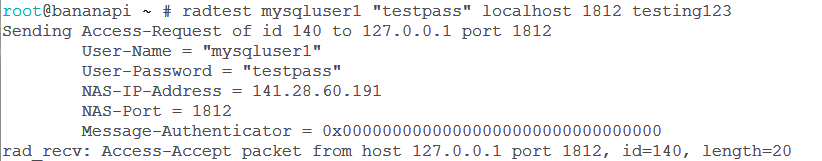
\includegraphics[width=\textwidth]{pictures/Tom/Radius2}
\caption{Radius Test}
\end{figure}
\newpage
\subsection{Inbetriebnahme von FreeRADIUS2 auf OpenWRT}
1. Installation des FreeRADIUS2 mit den üblichen Paketen die von verschiedenen anderen Paketen
benutzt werden:
\begin{lstlisting}
> opkg install freeradius2 freeradius2-common freeradius2-utils
Unknown package 'freeradius2'.
Unknown package 'freeradius2-common'.
Unknown package 'freeradius2-utils'.
Collected errors:
* opkg_install_cmd: Cannot install package freeradius2.
* opkg_install_cmd: Cannot install package freeradius2-common.
* opkg_install_cmd: Cannot install package freeradius2-utils.
\end{lstlisting}
-> Hat nicht funktioniert, auch nach halbstündiger Investigation konnte keine Lösung gefunden
werden, auch mit
\begin{lstlisting}
> opkg search freeradius2
> opkg info freeradius2
\end{lstlisting}
konnten keine Informationen über das Paket ermittelt werden. Schlussendlich konnten die Pakete
über das Web-Interface installiert werden, dort klappte es auf Anhieb (mit den gleichen
Bezeichnern)\\
~\\
2. Installation der FreeRADIUS2 Pakete für die MYSQL Unterstützung (+ Packet für Logging):
\begin{lstlisting}
> opkg install freeradius2-mod-sql freeradius2-mod-sql-mysql freeradius2-mod-sqllog
\end{lstlisting}
Nun sind die benötigten Pakete installiert.\\
\newpage
Die Ausgabe nach der Installation sieht folgendermaßen aus:
\begin{lstlisting}
nstalling freeradius2 (2.2.8-2) to root...
Downloading file:///etc/packages/packages/freeradius2_2.2.8-2_sunxi.ipk.
Installing freeradius2-common (2.2.8-2) to root...
Downloading file:///etc/packages/packages/freeradius2-common_2.2.8-2_sunxi.ipk.
Configuring freeradius2-common.
Configuring freeradius2.
ifconfig: br-lan: error fetching interface information: Device not found
ifconfig: br-lan: error fetching interface information: Device not found
radiusd: Invalid IP Address or hostname "-p"
\end{lstlisting}
Mit br-lan ist hier das sogenannte „bridged lan virtual interface“ gemeint (liegt daran dass es
standardmäßig so vorkonfiguriert ist).\\
Beim Versuch FreeRADIUS2 im Debugging-Modus zu starten kommt:\
\begin{lstlisting}
> radiusd -X
radiusd: FreeRADIUS Version 2.2.8, for host arm-openwrt-linux-gnu, built on Oct 3 2016 at 22:22:30
Copyright (C) 1999-2015 The FreeRADIUS server project and contributors.
There is NO warranty; not even for MERCHANTABILITY or FITNESS FOR A PARTICULAR PURPOSE.
You may redistribute copies of FreeRADIUS under the terms of the GNU General Public License.
For more information about these matters, see the file named COPYRIGHT.
Starting - reading configuration files ...
including configuration file /etc/freeradius2/radiusd.conf
including configuration file /etc/freeradius2/clients.conf
including files in directory /etc/freeradius2/modules/
including configuration file /etc/freeradius2/eap.conf
Unable to open file "/etc/freeradius2/eap.conf": No such file or directory
Errors reading or parsing /etc/freeradius2/radiusd.conf
\end{lstlisting}
EAP ist das Extensible Authentication Protocol, ein allgemeines Authentifizierungsprotokoll. Also
wurden die noch benötigten FreeRADIUS2 Abhängigkeiten Installiert:
\begin{lstlisting}
> opkg install freeradius2-mod-chap freeradius2-mod-detail freeradius2-mod-eap freeradius2-mod-eap-md5 freeradius2-mod-eap-mschapv2 freeradius2-mod-eap-peap freeradius2-mod-eap-tls freeradius2-mod-eap-ttls
freeradius2-mod-exec freeradius2-mod-files freeradius2-mod-logintime
freeradius2-mod-mschap freeradius2-mod-pap freeradius2-mod-passwd
freeradius2-mod-preprocess freeradius2-mod-radutmp
\end{lstlisting}
3. Installation des MYSQL-Servers
\begin{lstlisting}
> opkg install mysql-server
Installing mysql-server (5.1.73-1) to root...
Downloading file:///etc/packages/packages/mysql-server_5.1.73-1_sunxi.ipk.
Installing libmysqlclient (5.1.73-1) to root...
Downloading file:///etc/packages/packages/libmysqlclient_5.1.73-1_sunxi.ipk.
Configuring libmysqlclient.
Configuring mysql-server.
/etc/init.d/mysqld: Error: datadir '/mnt/data/mysql/' in /etc/my.cnf
doesn't exist
\end{lstlisting}
Nach einiger Zeit stieß ich im Internet auf vergleichbare Probleme und es gab einen Work-Around
mit dem der MYSQL-Server sich schließlich doch installieren lies.\\
~\\
4. Einrichtung einer Zertifikatskette für das EAP
\begin{lstlisting}
>opkg install openssl-util
\end{lstlisting}
->Erstellung der Zertifikatskette mit OpenSSL (...)\\
\newpage
5. Bevor man allerdings mit der Konfiguration beginnt, sollte man jedoch den Radius-Daemon
stoppen: Über das Web-Interface LuCi unter dem Menüpunkt „System“ ->„Startup“ wird der
radiusd deaktiviert („disable“) und erstmal vom automatischen Starten beim Booten
ausgenommen. Für Test- und Debuggingzwecke empfiehlt es sich außerdem, den Radius Server
umzukonfigurieren, sodass dieser auch auch auf Localhost horcht und nicht nur auf die IP Adresse
im Netzwerk. Dafür editiert man die Datei
\begin{lstlisting}
> vim /etc/init.d/radiusd
\end{lstlisting}
und ersetzt die Zeile 17
\begin{lstlisting}
radiusd -i $IPADDR -p 1812,1813 $OPTIONS
\end{lstlisting}
durch
\begin{lstlisting}
radiusd $OPTIONS
\end{lstlisting}













\section{Captive Portal}

\subsection{Algemeines}
Als Captive Portal (zu deutsch etwa „Umleitung auf ein Web-Portal“) wird eine Website bezeichnet,
die dafür verwendet wird Authentifizierungen durchzuführen, meistens findet sie in WLANs
Einsatz. In unserem Fall dient sie dem Login auf einer HTTP-Seite um sich beim RADIUS-Server
einzuloggen. \cite{chilli0}

\subsection{Funktionsweise}
Prinzipiell ist die Funktionsweise relativ simpel. Man benötigt lediglich einen Webserver und eine
Firewall, in unserem Fall Apache2 und iptables. Wenn nun ein Benutzer in ein WLAN-Netzwerk
möchte, wird erst einmal der komplette Netzwerkverkehr ignoriert, bis er einen Browser öffnet.
Dieser Zugriff wird immer auf das Captive Portal weitergeleitet, sodass der Benutzer immer zu der
Login-Seite kommt. Je nach Anwendungsfall können dort dann auch Bezahlsysteme implementiert
werden oder Nutzungsbedingungen die akzeptiert werden müssen.\\
Es gibt verschiedene Möglichkeiten wie die Umleitung von Statten gehen kann, durchgesetzt hat
sich aufgrund verschiedener sicherheitstechnischer Aspekte die Umleitung via HTTP (direkte IP-
sowie DNS-Umleitungen sind aufgrund des dann nicht mehr gültigen DNSSEC-Zertifikats nicht
möglich). \cite{chilli1}
\newpage
\subsection{CoovaChilli}
Allgemeines:\\
CoovaChilli ist ein open-source Tool das unter der GNU General Public License 3 veröffentlich wurde und frei zugänglich ist. Es bietet eine Zugriffskontrolle als Captive Portal und liefert die dafür benötigten HTML/CSS/Javascript Dateien. Es basiert auf dem mittlerweile nicht mehr unterstützten Projekt CoovaSpot und funktioniert mit dem RADIUS-Protokoll.\\
~\\
Funktionsweise:
\begin{figure}[ht]                                                                              
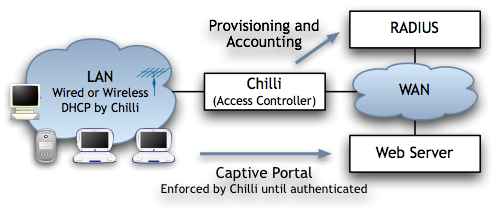
\includegraphics[width=\textwidth]{pictures/Tom/Chilli}
\caption{CoovaChilli Funktionsweise}
Quelle: \cite{chilli2}
\end{figure}
~\\
Wie in der Abbildung oberhalb zu erkennen bildet CoovaChilli die Instanz zwischen dem Access-
Point des Netzwerks und der Netzwerkinfrastruktur dahinter (in unserem Fall laufen Netzwerk-
Access-Server, also dem WLAN-AP, CoovaChilli und der RADIUS-Server auf der gleichen Maschine).
Will ein Benutzer nun ins Internet verbindet er sich wahlweise per LAN oder WLAN mit dem AP,
ruft den Browser auf und wird auf das Captive Portal auf dem Webserver weitergeleitet. Beim
Login kommuniziert CoovaChilli mit dem RADIUS-Server, bei erfolgreichem Login wird der
Internetzugang für den Benutzer freigegeben.
\newpage
Installation:\\


\chapter{Benutzeranleitung BananaPi}

\section{Pi Hoch- und Herunterfahren}
Um den Pi Hochzufahren, muss lediglich das Netzteil eingesteckt werden:\\
1. Netzteil in Steckdose einstecken\\
2. Micro-USB Port an den äußeren Port des Pis anschließen. Der andere Port ist nur für OTG!\\
~\\
Um den Pi Herunterzufahren muss benötigt man Zugriff auf die Kommandozeile\\
1. Pi an Tastatur und Bildschirm anschließen || SSH-Verbindung zum Pi aufbauen\\
2. Anmelden (User: root / Passwort: bananapi)\\
3. shutdown -h 0 eingeben und mit ENTER bestätigen\\

\section{Verbindung über SSH}
Um eine Verbindung über SSH aufzubauen wird folgendes benötigt:\\
~\\
- Putty (Windows)\\
- ssh-Packet (Linux)\\
- Netzwerkverbindung\\
~\\
Um eine Verbindung aufzubauen muss der Pi hochgefahren sein und über den Wan-Port an ein Netzwerk angeschlossen sein.
\newpage
\subsection*{Windows:}
1. Putty öffnen\\
2. Hostnamen armbian.bananapihfu.tk angeben
\begin{figure}[ht]
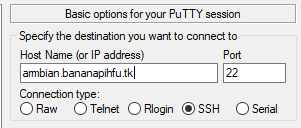
\includegraphics[width=.6\textwidth]{pictures/Jonas/Anleitung/BILD1}
\caption{Eingabe des Hostnamens}
\end{figure}
3. Durch Klick auf „Open“ Verbindung aufbauen -> Terminal öffnet sich
\begin{lstlisting}
login as: root
password: bananapi
\end{lstlisting}
4. Verbindung erfolgreich!

\subsection*{Linux:}
1. Terminal öffnen\\
2. Folgenden Befehl eingeben:
\begin{lstlisting}
ssh root@armbian.bananapihfu.tk
\end{lstlisting}
3. Passwort eingeben:
\begin{lstlisting}
password: bananapi
\end{lstlisting}
4. Verbindung erfolgreich!
\newpage
\section{Lan, Wlan und Vlans}
\subsection*{Übersicht Vlans:}
Der Pi besitzt 4 Lan Ports und einen Wlan Access-Point.\\
~\\
\begin{tabular}{r l}
Vlan 1:   & \\
	- & Internetzugriff\\
	- & Lan 1 + Lan 2\\
	- & Gateway:192.168.1.1\\
Vlan 2:   & \\
	- & Kein Internetzugriff\\
	- & Lan 3 + Lan 4\\
	- & Gateway:192.168.2.1\\
Vlan 3:   & \\
	- & Internetzugriff\\
	- & WLAN AP\\
	- & Gateway:192.168.3.1\\
\end{tabular}

\subsection*{Wlan:}
Der Pi besitzt einen Wlan-AP, über welchen eine Internetverbindung möglich ist. Lokal ist jedoch nur Zugriff auf Geräte im Vlan 3 möglich.
\begin{figure}[ht]

\includegraphics[width=.4\textwidth]{pictures/Jonas/Anleitung/BILD2}
\caption{Die SSID des AP}
\end{figure}
Um eine Verbindung zum AP herzustellen muss folgendermaßen Vorgegangen werden:\\
\begin{tabular}{l l}
1. & Wlan Übersicht am Client Gerät öffnen und nach APs suchen\\
   & a. The BananaPi Project auswählen\\
   & b. WPA/WPA2 PSK auswählen\\
   & c. Passwort: bananapi\\
2. & Verbindung hergestellt\\
\end{tabular}

\subsection*{Lan:}
Der Pi besitzt insgesamt 5 Lan-Ports. Einer davon ist der WAN-Port, welcher an ein externes Netzwerk angeschlossen wird. Die vier restlichen Ports werden über den Pi geroutet und sind in Vlans unterteilt (siehe Übersicht Vlans).

\section{Samba}
\subsection*{Verbindung aufbauen}
Mit Samba können Dateien zwischen dem Pi und einem anderen Gerät ausgetauscht werden.\\
Um den Samba-Share im am eigenen PC einzubinden muss folgendes gemacht werden:\\
~\\
\begin{tabular}{r l}
Windows:& \\
1. & Ausführen-Dialog aufrufen mit Win + R\\
2. & \textbackslash \textbackslash armbian.bananapihfu.tk\textbackslash samba eingeben und mit ENTER bestätigen\\
3. & Login Fenster öffnet sich\\
	& a. Login: sambausr\\
	& b. Passwort: bananapi\\
	& \\
Linux: & \\
1. & smbclient installieren:\\
	& a. sudo apt-get update\\
	& b. sudo apt-get install smbclient\\
2. & Verbindung aufbauen:\\
	& a. smbclient \textbackslash \textbackslash armbian.bananapihfu.tk /samba -U sambausr\\
	& b. Passwort eingeben: bananapi\\
	& \\
MacOSX: & \\
1. & Im Finder mit Server verbinden (Command + K)\\
2. & Serveradresse angeben:\\
	& a. smb://armbian.bananapihfu.tk/samba\\
3. & Verbinden als Registrierter Nutzer:\\
	& a. Name: sambausr\\
	& b. Passwort: bananapi\\
\end{tabular}

\section{Mailserver}
Um auf die Mails zuzugreifen, muss man https://www.google.com/gmail besuchen und sich mit folgenden Benutzerdaten anmelden:\\
- Email: bananapihfu\\
- Passwort: 63!gr\&8FJZdd\\
~\\
Um die Emails über einen Mail-Client aufzurufen, kann die Anleitung von Google zur Hand genommen werden:\\
https://support.google.com/mail/answer/7126229?hl=en

\section{Domainverwaltung}
\subsection*{Ni-IP}
Um die Dynamische DNS bei No-IP zu verwalten muss no-ip.com besucht werden:
- Login: bananapihfu\\
- Passwort: BananaPhone
\begin{figure}[ht]
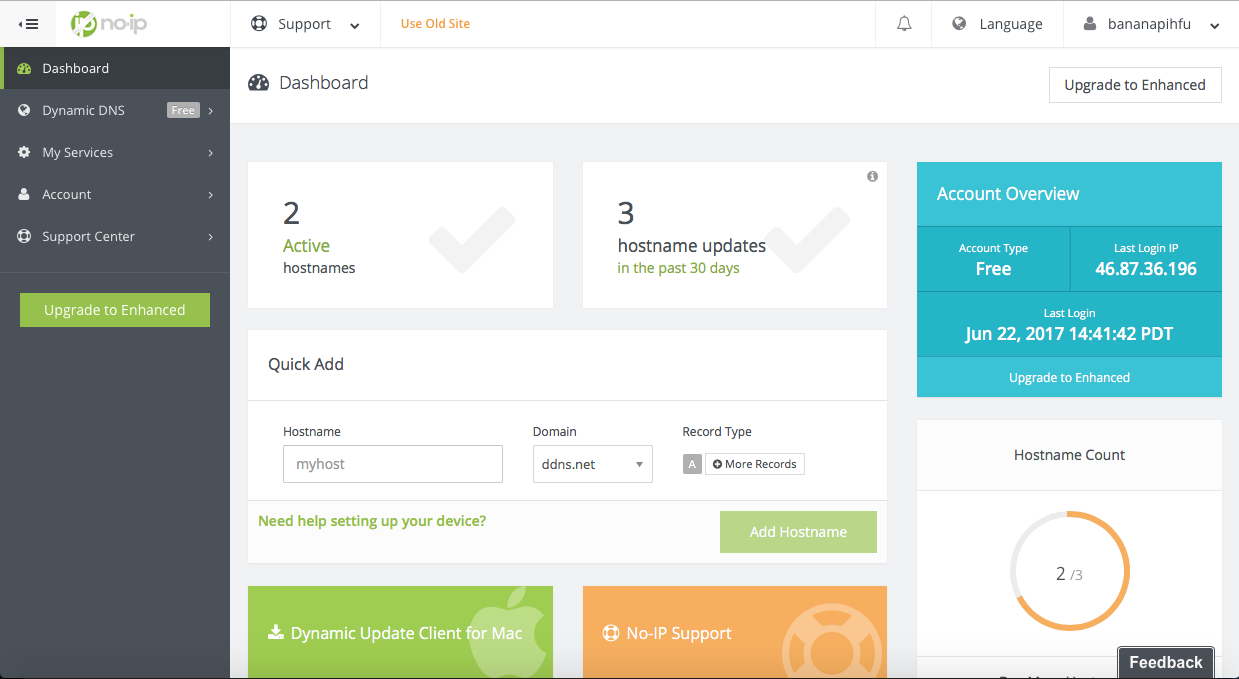
\includegraphics[width=\textwidth]{pictures/Jonas/Anleitung/BILD3}
\caption{No-IP Startseite}
\end{figure}
\newpage
\subsection*{Freenom.com}
Über Freenom wurde die kostenfreie Domain bananapihfu.tk gebucht.\\
Login: bananapihfu@gmail.com\\
Passwort: bananapi
\begin{figure}[ht]
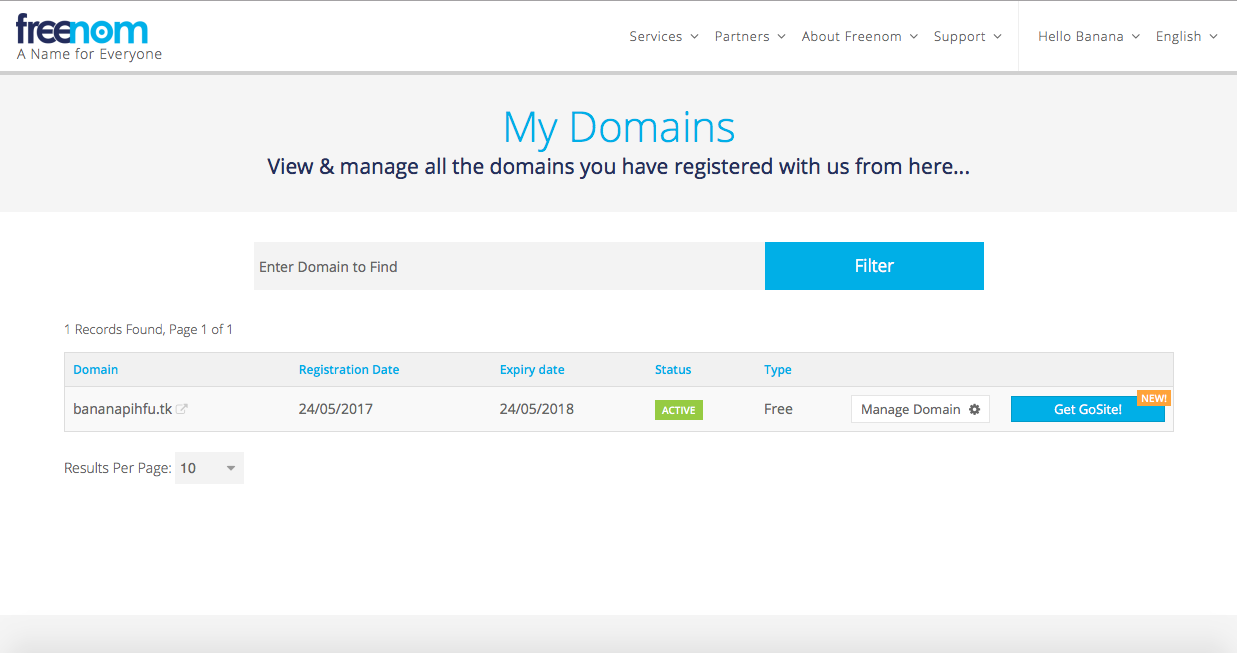
\includegraphics[width=\textwidth]{pictures/Jonas/Anleitung/BILD4}
\caption{Freenom Domainverwaltung}
\end{figure}

\subsection*{CloudFlare}
Über CloudFlare werden die DNS-Einträge der Domain verwaltet:\\
Login: bananapihfu@gmail.com\\
Passwort: k\%KKx!HkNW23
\begin{figure}[ht]
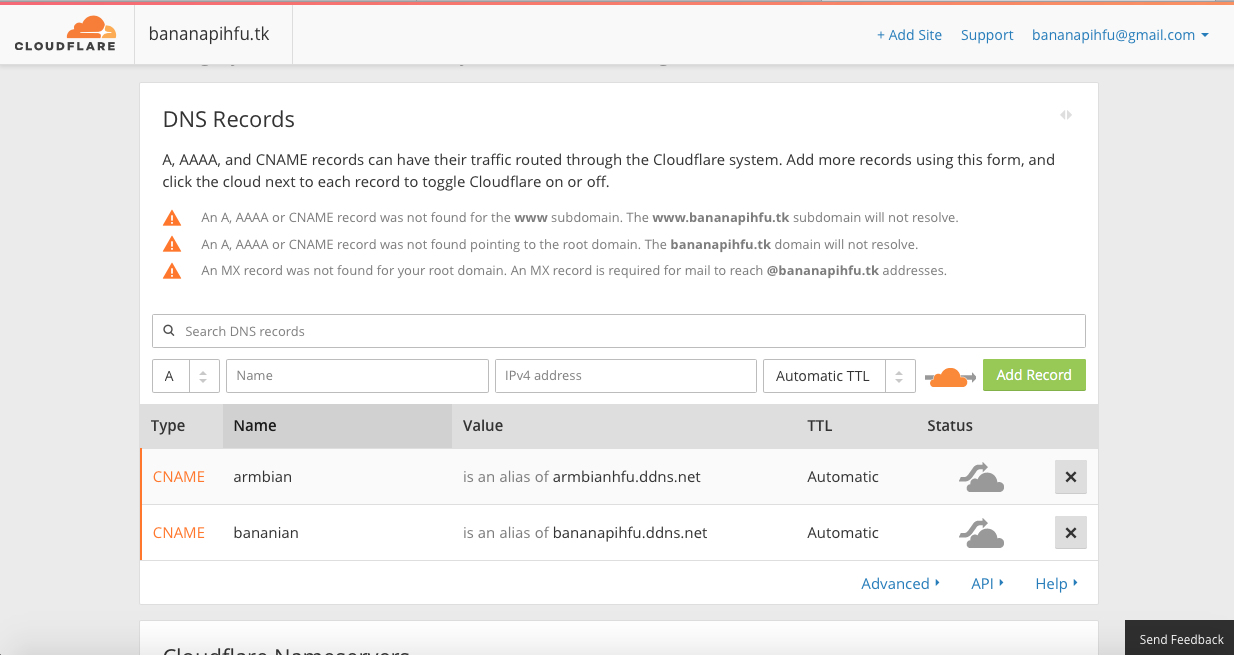
\includegraphics[width=\textwidth]{pictures/Jonas/Anleitung/BILD5}
\caption{Cloudflare DNS}
\end{figure}

\section{Backup und Restore}
Das Backup wird über zwei Skripte gestartet, welche in den Verzeichnissen /etc/cron.weekly/ und /etc/cron.monthly/ liegen. Das Backup wird somit regelmäßig ausgeführt.\\
~\\
Manuelles Backup\\
Sollte man ein aktuelles Backup benötigen, kann man das Backup-Script manuell ausführen:
\begin{lstlisting}
bash /etc/cron.weekly/Backup_Weekly
\end{lstlisting}
Hierbei wird das Backup unter /mnt/SSD/Backup\_Weekly gespeichert.\\
Zur Archivierung des Backups, kann auch das Backup\_Monthly aufgerufen werden:
\begin{lstlisting}
bash /etc/cron.monthly/Backup_Monthly
\end{lstlisting}
Dieses Skript speichert dann das Wöchentliche Backup unter /mnt/SSD/Backup\_Monthly als tar-Archiv.

\section{Statusanzeige}
Die Statusanzeige wird bei Systemstart geöffnet, da das Skript für diese unter /etc/init.d/ abgelegt ist. Das Skript baut eine tmux-Session auf, welche mit folgendem Befehl aufgerufen werden kann:
\begin{lstlisting}
tmux attach 
\end{lstlisting}
Beendet wird die Session mit folgender Tastenkombination:

\begin{lstlisting}
CTRL + D
\end{lstlisting}













\chapter{Projektbewertung}
Die technischen Herausforderungen des Projekts waren für alle Teilnehmer eine spannende und lehrreiche Erfahrung. Durch die Umsetzung der verschiedenen Implementationsziele auf der gegebenen eingebetteten Plattform können alle Projektteilnehmer einen großen Zugewinn an fachspezifischen Wissen verzeichnen.\\
Mit den wöchentlichen Projekttreffen war es möglich, frühzeitig auf aktuelle Probleme zu reagieren und Lösungsansätze gemeinsam zu erörtern.\\
Aufgrund des Wechsels von Bananian auf Armbian wurde der Zeitplan des Projekts  teils weit zurückgeworfen. Weniger vorweisbare Projekt-Ergebnisse und kleinere Entwicklungsschritte waren die Folge, da Kernfunktionen wie die Switcharchitektur des Banana Pi komplett neu entwickelt werden mussten. Zudem wirkten sich Updates des Betriebssystems teils deutlich auf die Verlässlichkeit und Bedienbarkeit des Geräts aus, was mutmaßlich dem noch unausgereiften Betriebssystem geschuldet ist, das sich zum Zeitpunkt des Projekts in einer sehr aktiven Entwicklungsphase befindet.\\

\chapter{Teilnehmer und Rollenverteilung}
Die Rollen der studentischen Projektteilnehmer wurden wie folgt aufgeteilt:\\\\
\begin{tabular}{l l}
Name & Hauptrolle \\
\hline
Bastian & - Projektleiter\\
	& - Entwicklung Backup Skripte\\
	& - Entwicklung Displaystatusanzeige\\
\hline
Jonas	& - Implementierung Mail-Server\\
	& - Implementierung Samba-Server\\
	& - Implementierung DDNS\\
\hline
Tom	& - Implementierung einer WLAN-Benutzerverwaltung\\
	& - Implementierung eines RADIUS-Server mittels CoovaChilli\\
\hline
Jakob	& - Erstellung der Dokumentation\\
	& - Untersuchung von IP-Fire als Alternatives Betriebssystem\\
\hline
Elias	& - Überprüfung des WLAN-Chips in Bananian\\
	& - Integration des WLAN und VLAN in Armbian\\
\end{tabular}
~\\~\\
Die Verteilung der Rollen und mancher Aufgabengebiete änderte sich im Verlauf des Projekts. Die hier dargestellte Unterteilung bezieht sich auf den Stand zum Semesterende.


\chapter{Ausblick}



% Schalgwortverzeichnis (Index)
%\printindex

% Literaturverzeichnis
\singlespacing
\bibliographystyle{plain}
\bibliography{bibtex}

% Eidesstattliche Erklärung
\chapter*{Eidesstattliche Erklärung\markboth{Eidesstattliche Erklärung}{}}
% Eintrag in das Inhaltsverzeichnis 
\addcontentsline{toc}{chapter}{Eidesstattliche Erklärung}

Ich versichere, dass ich die vorstehende Arbeit selbständig verfasst und hierzu
keine anderen als die angegebenen Hilfsmittel verwendet habe. Alle Stellen der Arbeit die 
wörtlich oder sinngemäß aus fremden Quellen entnommen wurden, sind als solche kenntlich gemacht.
\\
\\
Die Arbeit wurde bisher in gleicher oder ähnlicher Form in keinem anderen
Studiengang als Prüfungsleistung vorgelegt oder an anderer Stelle
veröffentlicht.
\\
\\
Ich bin mir bewusst, dass eine falsche Erklärung rechtliche Folgen haben kann.

\vspace*{1.5cm} \par
\line(1,0){200} \par
\docOrt, den  \docAbgabedatum


\appendix
% Hier können Anhaenge angefuegt werden

\end{document}      
